 \documentclass[25pt, a0paper, portrait, margin=0mm, innermargin=15mm,
     blockverticalspace=15mm, colspace=12mm, orientation=landscape]{tikzposter} %Default values for poster format options.

\tikzposterlatexaffectionproofon 
\usepackage[utf8]{inputenc}
\usepackage{alltt}
\usepackage{amsmath}
\usepackage{enumitem}
\usepackage{bbding}
\usepackage{tikz}
\usepackage{graphicx}
\usepackage{caption}
\usepackage{float}
\floatstyle{boxed}
\restylefloat{figure}


 % Title, Author, Institute
\title{\LARGE Scene Recognition with Convolutional Neural Networks}
\author{Alexander Seewald}
\institute{Computer Vision Lab at Indiana University Bloomington}
\date{Jul. 21st, 2014}

 % -- PREDEFINED THEMES ---------------------- %
 % Choose LAYOUT:  Default, Basic, Rays, Simple, Envelope, Wave, Board, Autumn, Desert,
 \usetheme{Simple}
\usecolorstyle[colorPalette=BrownBlueOrange]{Germany}


 \begin{document}

     \maketitle

     \begin{columns}%blocks will be placed into columns
         \column{.40}
         \block[roundedcorners=40]{Neural Networks}{
      \usetikzlibrary{arrows}
       \hspace{-3em}{0}{
       \begin{tikzpicture}[->,>=stealth',shorten >=1pt,auto,node distance=7cm,
         thin,main node/.style={circle,fill=blue!20,draw,font=\sffamily\bfseries}]
        \node [main node] (1) {tanh};
        \node [main node] (2) [below of=1] {sig};
        \node [main node] (0) [left of=2] {x};
        \node [main node] (3) [below of=2] {relu};
        \node [main node] (4) [below of=3] {abs};
        \node [main node] (5) [right of=1] {relu};
        \node [main node] (6) [right of=2] {sig};
        \node [main node] (7) [right of=3] {tanh};
        \node [main node] (8) [right of=4] {abs};
        \node [main node] (9) [right of=7] {loss};
        \node [main node] (10) [right of=9] {y};

        \path[ every node]
            (0) edge node [right] {$w_{i-1,j}$} (1)
                edge node [right] {$w_{i-1,j+1}$} (2)
                edge node [right] {$w_{i-1,j+2}$} (3)
                edge node [right] {$w_{i-1,j+3}$} (4)
            (1) edge node [right] {} (5)
                edge node [right] {} (6)
                edge node [right] {} (7)
                edge node [right] {} (8)
            (2) edge node [right] {} (5)
                edge node [right] {}  (6)
                edge node [right] {}  (7)
                edge node [right] {}  (8)
            (3) edge node [right] {} (5)
                edge node [right] {}  (6)
                edge node [right] {}  (7)
                edge node [right] {}  (8)
            (4) edge node [right] {}   (5)
                edge node [right] {}  (6)
                edge node [right] {}  (7)
                edge node [right] {}  (8)
            (5) edge node [right] {$w_{i+4,j+4}$} (9)
            (6) edge node [right] {$w_{i+5,j+4}$} (9)
            (7) edge node [right] {$w_{i+6,j+4}$} (9)
            (8) edge node [right] {$w_{i+7,j+4}$} (9)
            (9) edge node [right] {} (10);
       \end{tikzpicture}}

         A fully connected neural network with a single hidden layer.
     }
     \block{Mathematical Techniques}{
        \begin{align}
        W &= { w_{i,j}, b }  &  y_0 &= (\vec{x},t)   &     y_i &= \sum \limits_j w_{i,j} y_i-1,j \\
        sig(x) &= \frac{1}{1 - e^{-x}}  &  tanh(x) &= \frac{e^x - e^{-x}}{e^x + e^{-x}} & relu(x) &= 
        \begin{cases} 
        0 & \text{if } x < 0 \ &
        x & \text{if } x \geq 0
        \end{cases} \\
        E(y,t) &= \frac{1}{2}(t - y)^2   &   G &= \frac{\partial E}{\partial w_{i,j}} & \Delta w_{i,j} &= - \mu \frac{\partial E}{\partial w_{i,j}} 
        \end{align}
        
        \smallskip

\subsection*{A Basic Explanation of Forward Feed and Back Propagation (Training)}
        \hspace{2em} Initially, all weights are small random values. When input is run all the way through the neural network, the ground truth label $t$, the weights $w_{i,j}$, and the prediction $y_f$ are known. The error $E$ can be computed and, then, so can the partial derivative of the error with respect to each of the weights. The weights are then changed such that the error declines most steeply (opposite the direction of the gradient). Such a naive approach would obviously get into trouble with local minima; more advanced methods are discussed in the procedure section.

\subsection*{Convolutional Neural Networks (CNN)}
        \hspace{2em} CNNs are a generalization of the simple neural networks described above. They have the following features...
        \begin{itemize}[label= \small \EightFlowerPetalRemoved]
            \item Inner product layers, also known as fully connected layers, do what most people understand neural networks to do.
            \item Convolution layers perform a convolution operation with kernels such as...
                 \begin{pmatrix}
                  0 & -1 & 0 \\
                  -1 & 4 & -1 \\
                  0 & -1 & 0 \\
                 \end{pmatrix}
                 This has the effect of sharpening edges.
            \item Pooling layers homogenize a neighborhood to the value of a certain pixel, perhaps the pixel of maximum intensity and perhaps that of average intensity. Pooling reduces the computational complexity of the problem.
            \item Dropout layers randomly set an activation function's value to 0 every so often.
        \end{itemize}

\subsection*{Support Vector Machines}
    Like neural networks, SVMs store knowledge and define a loss function which training attempts to minimize. The difference is that SVMs' knowledge is a hypersurface that separates clustered data (which correspond to categories). Because SVMs are purely general purpose, they can be connected to neural networks as part of a prediction ensemble.  
     }

     \column{.32}
         \block{Why Snow?}{
        \hspace{2em}Snow's presence in digital images is physically similar to other phenomena, such as glare and overexposure. Where humans see a wintery scene that may trigger memories of cold and play, a naive computer program sees a region of highly saturated pixels. Humans' ease in classifying snow is based on a vast amount of knowledge about the world and the ability to pick up on context cues.

    \smallskip

        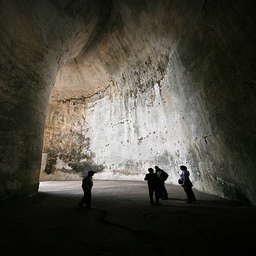
\includegraphics[width=0.5\linewidth]{images/deceptive_1.jpg}
        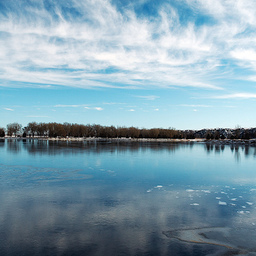
\includegraphics[width=0.5\linewidth]{images/deceptive_2.jpg}

        \hspace{2em}The reflected sunlight in the image on the left may look like snow to a machine, but is clearly a stone surface to a human can examine the whole scene. The image on the right could easily be interpreted as an upside down lake with snow on top and trees in the distance. However, humans can observe the symmetry between the trees and their reflection, identify the true lake line, and infer that the white fluff must be clouds. In order for computers to compete, an understanding of the scene must be had. Convolutional neural networks have been shown to have special promise in scene recognition \cite{scene}.
     }
        \block{Methods} {
        \hspace{2em}I trained many neural networks with a variety of initial learning rates, dynamic learning rate function types, and parameters to those dynamic functions. The idea is to characterize the best way to learn the binary snow classification problem.

        \hspace{2em}There are a number of design decisions to make. When doing back propogation weights may be updated as soon as their change in value due to a single image is computed, or the changes may be stored in an accumulator variable until 'N' images passing through (at which point all the changes will be applied at once). The latter approach is called batch learning. Because the first images have less of an undue influence, machine learning done in batches tends to generalize better. In addition to making intuitive sense, this is a well-documented result in the literature \cite{batch}.

        \hspace{2em}There exists some software called caffe that implements highly-flexible CNN forward feed and back propagation solvers \cite{caffe}. One simply specifies a network topology in a Google protocol buffer (see below for a sample) and can start experimenting.

\begin{center}
\scriptsize \texttt{
 layers \{ \\
 name: "conv2" \\
 type: CONVOLUTION \\
 bottom: "norm1" \\
 top: "conv2" \\
 blobs\_lr: 1 \\
 blobs\_lr: 2 \\
 weight\_decay: 1 \\
 weight\_decay: 0 \\
 convolution\_param \{ \\
 \hspace{3cm}     num\_output: 256 \\
 \hspace{3cm}     pad: 2 \\
 \hspace{3cm}     kernel\_size: 5 \\
 \hspace{3cm}     group: 2 \\
 weight\_filler \{ \\
 \hspace{6cm}     type: "gaussian" \\
 \hspace{6cm}     std: 0.01 \\
 \} \\
 bias\_filler \{ \\
  \hspace{6cm}    type: "constant" \\
 \hspace{6cm}     value: 1 \\
 \} \\
 \} \\
\}
}
\end{center}

\hspace{2em} Another method I used to recognize snow is to extract image features at various points in the network and pass the data off to an SVM for classification. Such an approach has been found to be successful \cite{features}. Results in these experiments are preliminary.
}
     \column {0.28}
     \block{Results}{
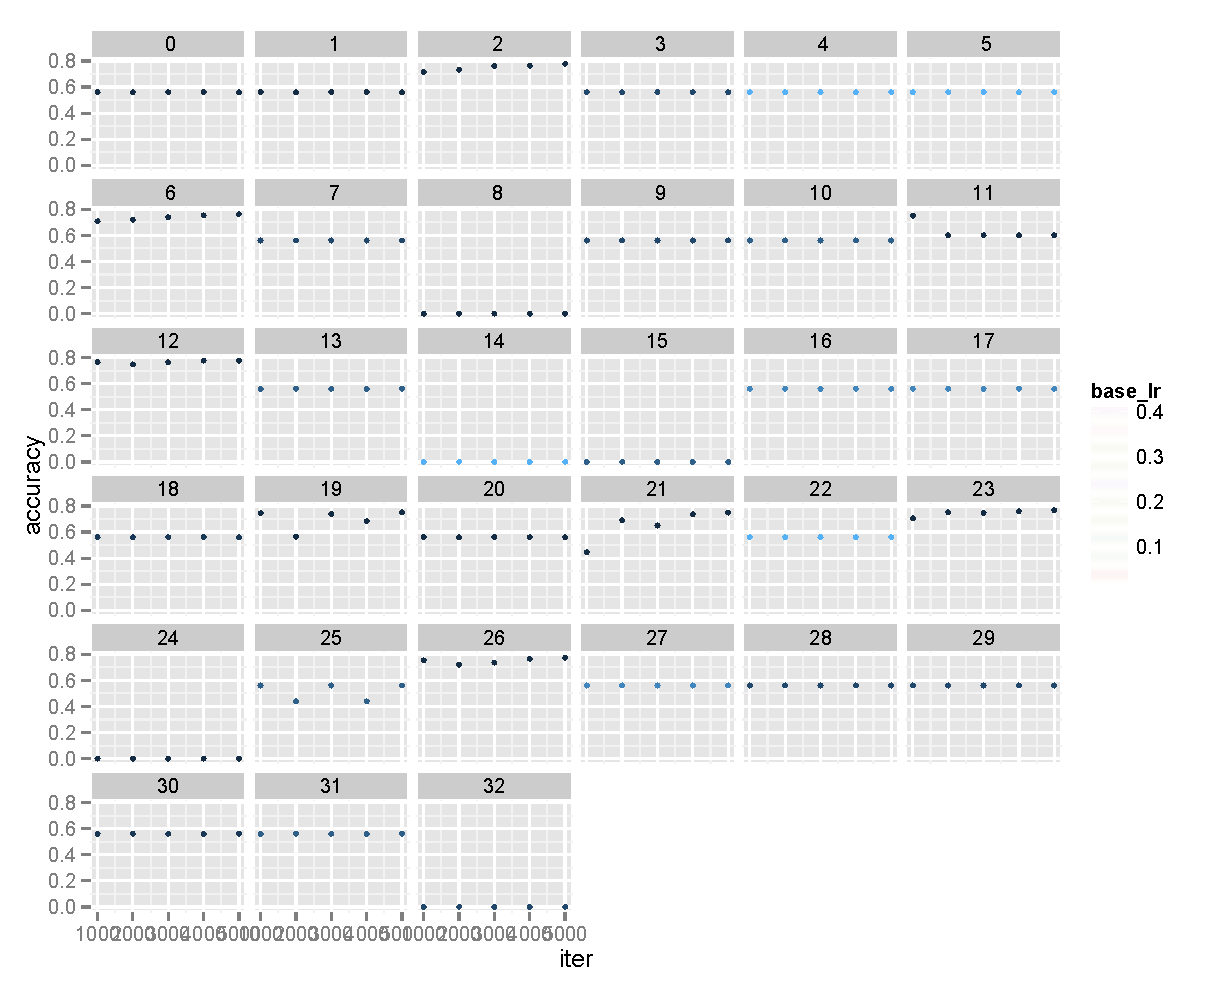
\includegraphics[keepaspectratio=true,scale=0.9]{images/plot_t.pdf}

\small \texttt{ggplot( data=the\_data, aes(x = iter, y = accuracy, colour = base\_lr)) + geom\_point() + facet\_wrap(~ set\_id)}

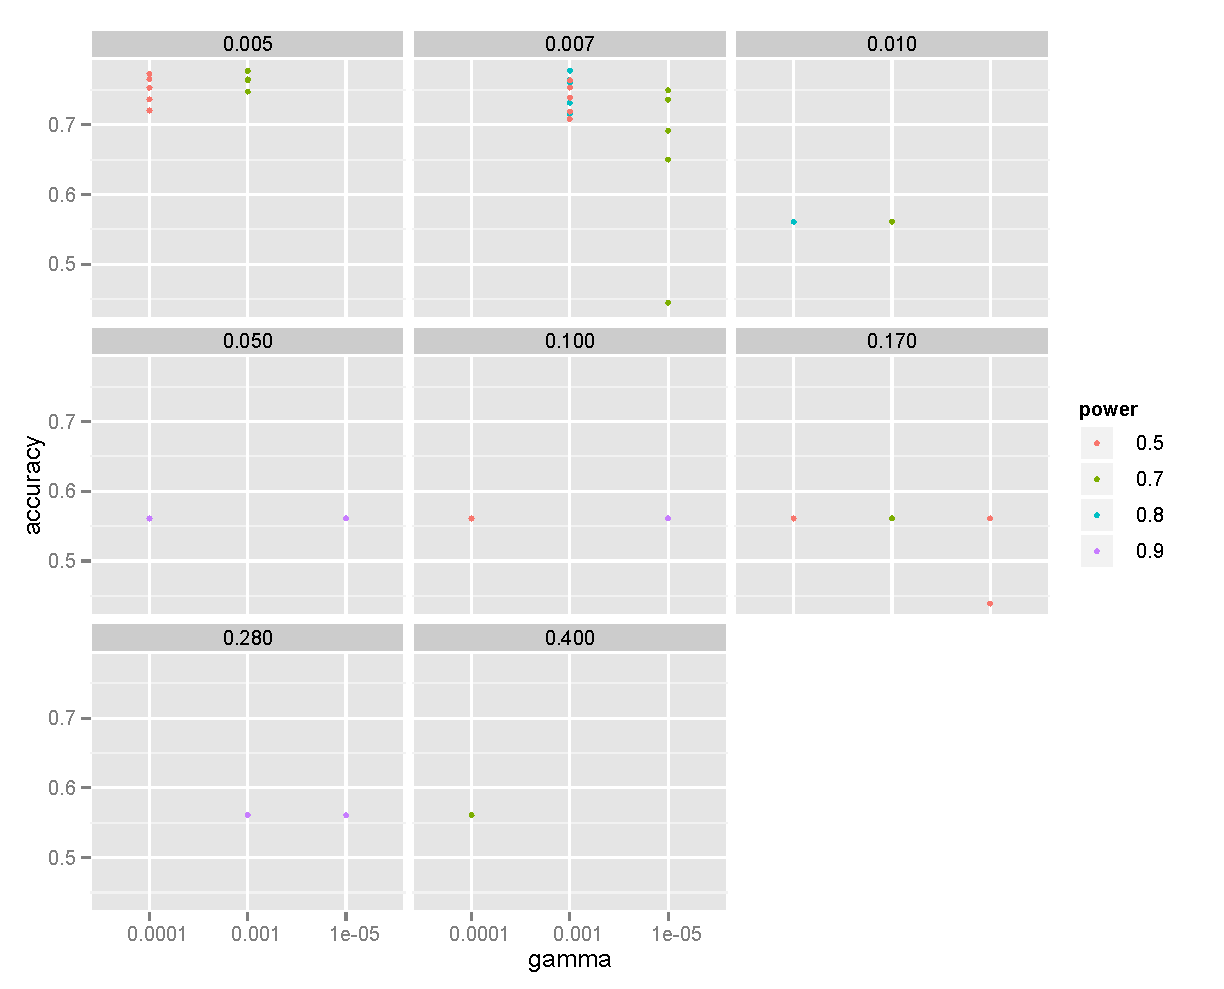
\includegraphics[keepaspectratio=true,scale=0.7]{images/plot_inv.pdf}

\small \texttt{ggplot(data=the\_data[the\_data\$base\_lr == lrs[i]], aes(x = gamma, y = accuracy, colour = power)) + geom\_point() + facet\_wrap(~ base\_lr)}

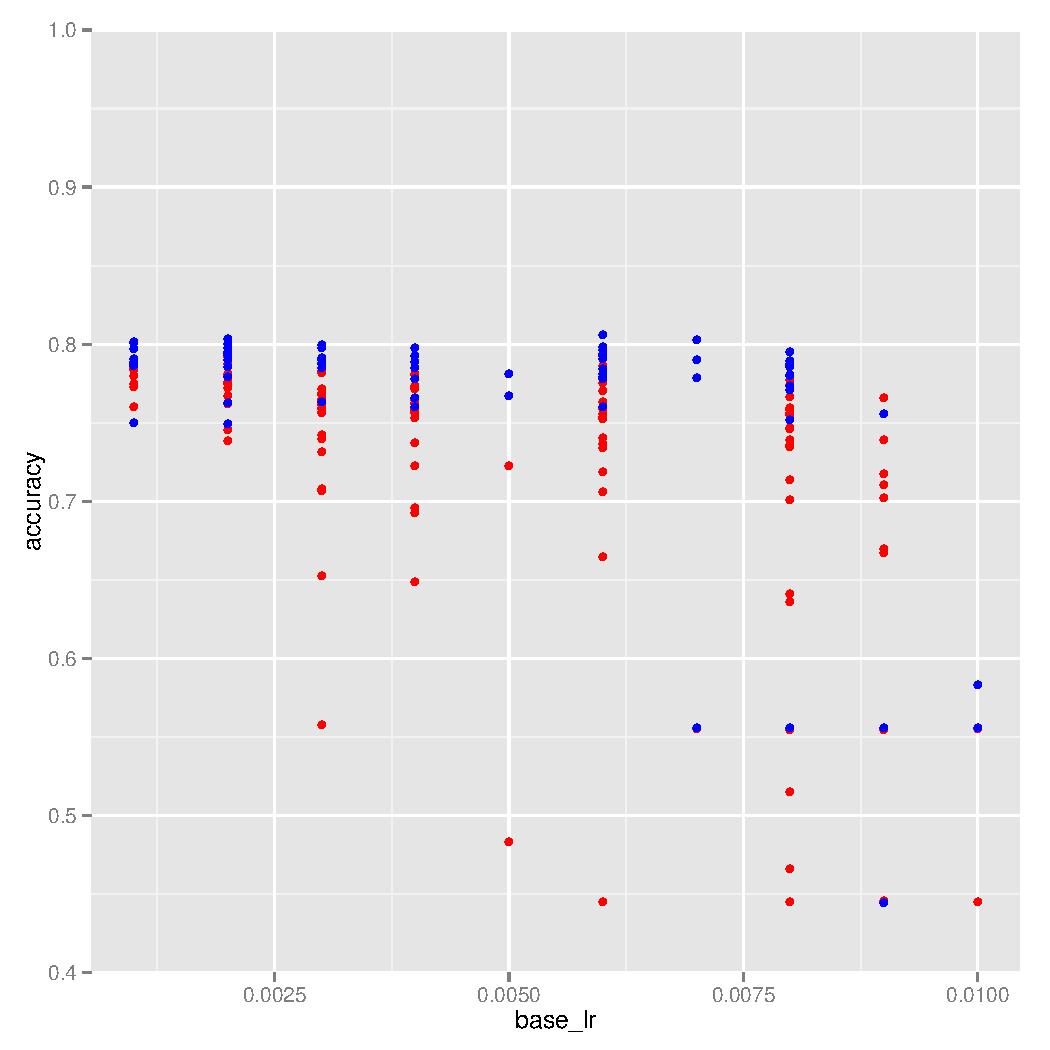
\includegraphics[keepaspectratio=true,scale=0.8]{images/plot_mean.pdf}

\small \texttt{ggplot() + geom\_point(data=no\_mean, aes(x = base\_lr, y = accuracy), colour='red') + geom\_point(data=yes\_mean, aes(x = base\_lr, y = accuracy), colour='blue') + coord\_cartesian(ylim = c(0.4,1.0))}
     }

     \block{Analysis}{

        \begin{enumerate}
            \item One starkly evident property of the data is that many of the models have the same exact predictive accuracy. These common values are 56\%, 63\%, and 80\%. This is most likely because there are a few local minima of the loss function somewhere in the parameter space that are hard to tunnel out of. Because the value of 56\% accompanies high initial learning rates, $\mu_0$, changing the weights too rapidly seems to have the effect of entirely skipping over the favorable values.
            \item Performance tends to be slightly better when the mean pixel intensity value for a given image is subtracted from every pixel value. This does not come as a surprise; it is a commonly used technique whose benefit is shown here.
            \item Classification accuracy can vary significantly over time. Good engineering practice is, then, to generate models at many points in the training and use the best one for discovery.
        \end{enumerate}

         \begingroup
         \fontsize{14pt}{16pt}\selectfont
         \begin{thebibliography}{5}
            \bibitem{scene}
              Aditya Khosla and Byoungkwon An and Joseph J. Lim and Antonio Torralba,
              Looking Beyond the Visible Scene.
              2014
            \bibitem{batch}
              Ofer Dekel,
              From Online to Batch Learning with Cutoff-Averaging.
              D. Koller and D. Schuurmans and Y. Bengio and L. Bottou,
              2008
            \bibitem{caffe}
              Yangqing Jia,
              Caffe: An Open Source Convolutional Architecture for Fast Feature Embedding.
              http://caffe.berkeleyvision.org/
              2013
           \bibitem{features}
             Oquab, Bottou, Laptev, Sivic,
             Learning and Transferring Mid-Level Image Represenations using Convolutional Neural Networks.
             2013
         \end{thebibliography}
         \endgroup

     }
     \end{columns}

     \block{\small Acknowledgements} {
         This work was supported in part by the National Science Foundation through CAREER award IIS-1253549 and through the FutureGrid project (ACI-0910812).
     }


 \end{document}




\endinput
%%
%% End of file `tikzposter-example.tex'.
